\documentclass[12pt]{article}

\usepackage{amssymb,amsmath,amsthm}
\usepackage{pgfplotstable,booktabs,longtable}
\usepackage{graphicx} % Package for including figures
%\usepackage{psfrag,color}

\title{Homework 3 \protect  \\(Math/CS 471)}

\author{Elijah Perez \protect \newline \\Natalie Chang}


\date{\vfill 9/30/2020}   



\begin{document}
	\maketitle
	\pagebreak
	\section{Introduction}
     This report explores two different ways of computing approximate integrals, and compares the results between the two. The methods belong to a class of Newton-Cotes quadrature rules. The main difference between the two methods is the placement of the nodes. The method used to complete this experiment can be found in the Methods section. The results of the experiment can be found in the Results section. The discussion of the results and any final remarks can be found in the Conclusion section.
     
	\section{Method}
	The integral that we will be approximating in order to show the difference between two numerical integration techniques is:
	\begin{equation}
		I = \int_{-1}^1  e^{cos(kx)} dx
	\end{equation}
	\begin{center}
	We will be approximating I when $k=\pi$ and $k=\pi^2$.
    \linebreak\\ 
	The two methods are:
	\end{center}
	Trapezoidal

	\begin{equation}
		\int_{X_L}^{X_R} f(x) dx \approx h(\frac{f(x_0) + f(x_n)}{2} + \sum_{i=1}^{n-1} f(x_i))
	\end{equation}
	\linebreak
	Gauss Quadrature 
	\begin{equation}
			\int_{X_L}^{X_R} f(z)w(z) dx \approx \sum_{i=0}^{n} \omega_i f(x_i)
	\end{equation}
	Here, $\omega_i$ is a weight. The nodes and weights are found using the Legendre polynomials.

	\section{Results}
	The following plot shows the convergence rate for each of the 4 cases by plotting the error against the number of iterations taken to reach the desired error tolerance of $10^{-10}$. 
	\pagebreak
	
\begin{figure}[h!]
	
	\centering
	
		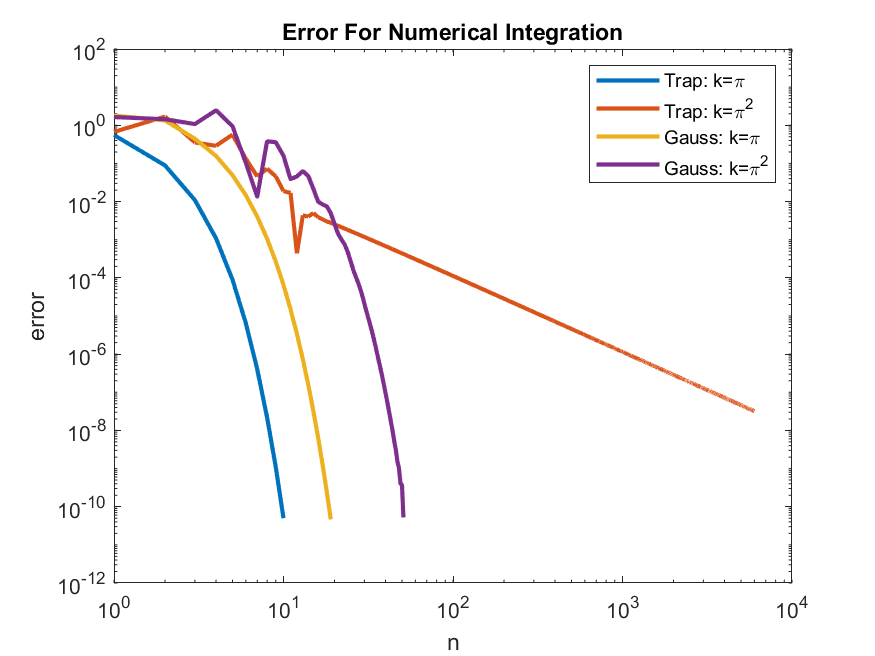
\includegraphics[width=\linewidth,height=100mm]{HW3_plot.png}	

	\end{figure}

From this graph, we can conclude the following convergence rates:
\\Trapezoidal $k = \pi$ is supergeometric
\\ Trapezoidal $k = \pi^2$ is algebraic
with order O($n^{-2}$)\\ Gauss $k = \pi$ is supergeometric
\\ Gauss $k = \pi^2$ is geometric
	
\pagebreak
	
	\section{Conclusion}
When $k = \pi$, we see the trapezoidal method performing at a superior rate. When integrating by the trapezoidal rule, the convergence is exponential for this case. This can be explained by the Euler-Maclaurin formula which shows that there is some p, depending on the function and step size (h), such that the terms past order p increase rapidly. Thus, when we expand the trapezoidal rule over some interval, the remainder terms of the Euler-Maclaurin formula become increasingly small. \\\\Both methods converge slower when considering the case of $k = \pi^2$. However, we can see that the Gauss Quadrature method still converges exponentially. This can be explained by the use of the weighted nodes. These weights are considered to be optimal and are chosen so that the order of the approximation to the weighted integral (3) is maximized. \\\\Overall, it can be concluded that both the Guass quadrature and Trapezoidal rules will approximate the integral with a very small error. Both are seen to be accurate. The convergence rate of the Gauss quadrature method is more stable, as the Trapezoidal rule experienced two very different convergence rates. In order to see this more thoroughly, this experiment can be repeated with a range of different functions.	

\end{document}  
